Rancangan integrasi dengan sistem FHIR dapat dilihat pada Gambar 4.6. Sistem ini akan terintegrasi dengan sistem FHIR untuk mendapatkan data login dari pasien. Data login ini kemudian akan digunakan sebagai input untuk melakukan analisis risiko autentikasi.
\begin{figure}[H]
    \centering
    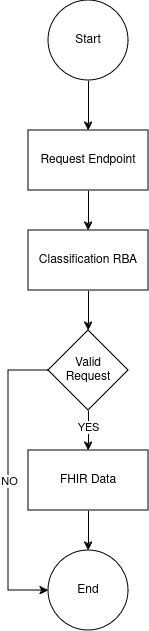
\includegraphics[width=0.2\textwidth]{BAB_TESIS/IMAGES/fhir_rba.drawio.png}
    \caption{Rancangan Integrasi Dengan Sistem FHIR}
    \label{fig:integrasi}
\end{figure}

Untuk melakukan integrasi dengan sistem FHIR, sistem ini akan menggunakan FHIR API. FHIR API adalah sebuah API yang digunakan untuk mengakses data dari sistem FHIR. FHIR API akan mengakses data dari sistem FHIR dengan menggunakan request dan response. 

Proses menentukan validitas proses FHIR terkait dengan kemampuan suatu sistem untuk mengakses data dalam format FHIR. Ini dapat diuji melalui keberhasilan proses klasifikasi autentikasi random forest. Proses tersebut melibatkan pembagian data menjadi data pelatihan dan data uji, diikuti oleh pelatihan model klasifikasi random forest menggunakan data pelatihan. Setelah itu, model tersebut dievaluasi menggunakan data uji untuk menilai performanya. Jika hasil dari model klasifikasi menentukan bahwa akses tersebut valid, maka akses ke data FHIR akan diberikan.